\begin{figure}[H]
    \centering
    \definecolor{coreorange}{RGB}{225,120,55}
    \definecolor{mantleblue}{RGB}{90,155,210}
    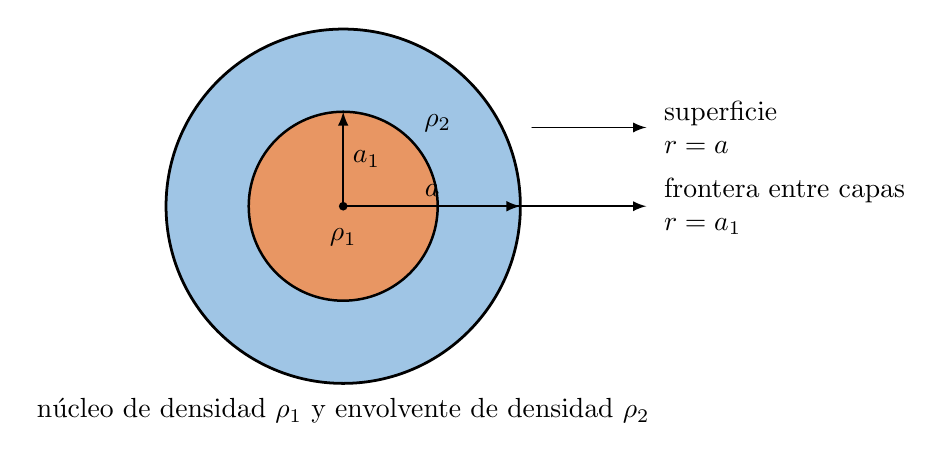
\begin{tikzpicture}[x=1cm,y=1cm,line cap=round,line join=round]
        \coordinate (O) at (4.25,2.55);

        \fill[mantleblue!58] (O) circle (2.25);
        \fill[coreorange!78] (O) circle (1.20);
        \draw[line width=1.0pt] (O) circle (2.25);
        \draw[line width=0.9pt] (O) circle (1.20);
        \fill (O) circle (0.055);

        \draw[-latex,line width=0.75pt] (O) -- ++(0:2.25);
        \node[above] at (5.38,2.55) {$a$};
        \draw[-latex,line width=0.75pt] (O) -- ++(90:1.20);
        \node[right] at (4.25,3.15) {$a_1$};

        \node at (4.25,2.15) {$\rho_1$};
        \node at (5.45,3.60) {$\rho_2$};

        \draw[-latex,line width=0.65pt]
            (6.65,3.55) -- (8.10,3.55);
        \node[right,align=left] at (8.20,3.55)
            {superficie\\$r=a$};

        \draw[-latex,line width=0.65pt]
            (5.48,2.55) -- (8.10,2.55);
        \node[right,align=left] at (8.20,2.55)
            {frontera entre capas\\$r=a_1$};

        \node[align=center] at (4.25,-0.05)
            {núcleo de densidad $\rho_1$ y envolvente de densidad $\rho_2$};
    \end{tikzpicture}
    \caption{Modelo del planeta esférico de dos capas del problema 2.}
\end{figure}
